\subsection{Problema 1}

\textit {“Desarrollo y explicación de problema 1 “Indicaciones al ejercicio en clase calcular el iva de 15\%, si las compras superan \textdollar2000 al cliente se agregar un descuento del 20\%, mostrar tanto el sueldo a ganar del vendedor y la factura de la venta de productos.”}

\textbf{Modelo}

Para desarrollar este ejercicio, se tienen 3 métodos en la clase del modelo.

\begin{center}
\begin{lstlisting}
  // Getter total ventas
  double get totalVentas => venta1 + venta2 + venta3;

  double calcularSueldo() {
    double sueldoBase = 36500;
    double comision = totalVentas * 0.12;
    return sueldoBase + comision;
  }

  double obtenerDescuento() {
    if(totalVentas >= 2000){
      return totalVentas * 0.20;
    }
    return 0;
  }
\end{lstlisting}
\end{center}

Las variables \lstinline{venta1}, \lstinline{venta2} y \lstinline{venta3} son atributos de la clase modal. Estas permiten obtener los valores del total de las ventas, un descuento si las ventas totales supera los \textdollar2000 y el sueldo del trabajador más su comisión del 12\% por cada venta.

\textbf{Controlador}

El controlador, toma este modelo y realiza las validaciones de texto correspondientes antes de ejecutar acciones sobre las variables numéricas de las ventas. En este método se retorna los valores respecto al total de las ventas, sueldo, descuento y el mensaje de error (en caso de haberlo).

\begin{center}
\begin{lstlisting}
  final billModel = BillModel(v1, v2, v3);
   final sueldo = billModel.calcularSueldo();
   final descuento = billModel.obtenerDescuento();

   return (billModel.totalVentas, sueldo, descuento, "");
\end{lstlisting}
\end{center}

\textbf{Vistas}

Dentro de la vista, una vez que se presiona el botón de calcular, se utiliza el controlador para mostrar obtener los resultados o los errores antes de realizar la acción. En caso de que todo fluya con normalidad, se pasan los datos a la ruta de resultados para mostrar los resultados en una nueva pantalla.

\begin{center}
\begin{lstlisting}
void _calcular() {
  final (totalVentas, sueldo, descuento, err) = mainctrl.calcularDatos(
      venta1ctrl.text,
      venta2ctrl.text,
      venta3ctrl.text,
  );

  // actualizar mensaje de error
  setState(() {
    msgErr = err;
  });

  // no mostrar pasar a la siguiente pantalla si hubo un error
  if(err != "") {
    return;
  }

  Navigator.pushNamed(
      context, "/bill/result",
      arguments: {
        'totalVentas': totalVentas,
        'sueldo': sueldo,
        'descuento': descuento,
      }
  );
}
\end{lstlisting}
\end{center}

Puesto que se mandaron argumentos en forma de clave valor, se realizaron colocaron los siguientes comandos para obtener cada uno de los argumentos en la vista de resutlados.

\begin{center}
\begin{lstlisting}
  @override
  Widget build(BuildContext context) {
    final args = ModalRoute.of(context)!.settings.arguments as Map<String, double>;

    final double totalVentas = args['totalVentas']!;
    final double sueldo = args['sueldo']!;
    final double descuento = args['descuento']!;
  }
\end{lstlisting}
\end{center}

\textbf{Ejecución}

De esta manera se pudo cumplir con el ejercicio propuesto, donde se toman 3 valores y con ellos se realizan varios cálculos mostrados en la siguiente pantalla:

\begin{figure}[H]
    \centering
    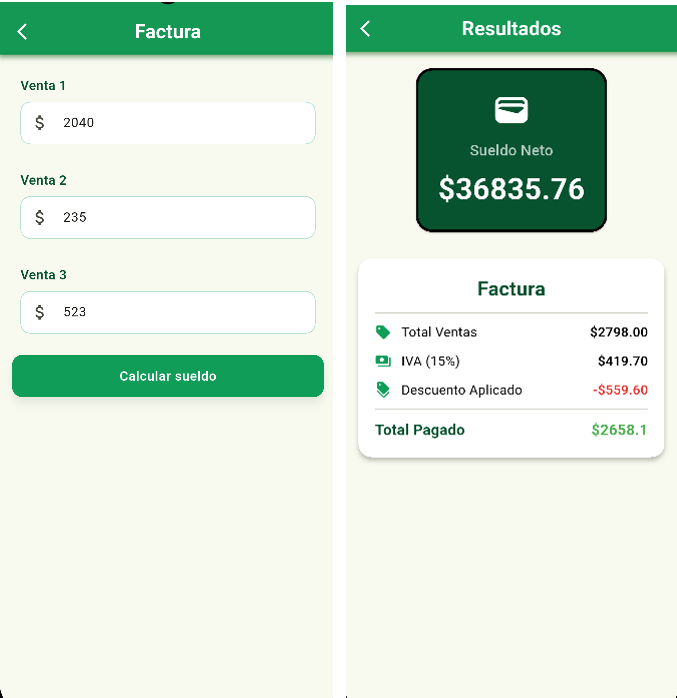
\includegraphics[width=0.8 \textwidth, height=10cm, keepaspectratio]{ejecucion_ej1.png}
    \caption{Ejecución ejercicio 1}
    \label{fig:ej1_ejecuccion}
\end{figure}